-\section{Coils alternatives}
This research was originally born from the willingness to explore the possibility of exploiting the technology of flexible coil inductors by using one produced by the research group Helmholtz-Zentrum Dresden-Rossendorf (HZDR) in Dresden, Germany \cite{HZDR}.
After testing this coil, we realized its limitations and decided to explore other alternatives.
For our research, we landed on Flexar coils, which as we discussed before are flexible PCB coils produced by the company \textbf{microbots} \cite{microbots}.
In this section, we will compare the Dresden coil with the Flexar coil, which is the one we chose to use in our research.

% -- Subsection 5.1
\subsection{Dresda coils}
The technology the HZDR team used to produce their coil is based on circuit inkjet printing.
Circuit inkjet printing consists of using a printer to deposit conductive ink on a substrate.
In this application, they used a flexible substrate to print the coil to allow it to be bent.
After printing the conductive ink is tinned to improve the conductivity of the coil and allow it to be soldered to other components.
\begin{figure}
    \centering
    \resizebox{0.5\textwidth}{!}{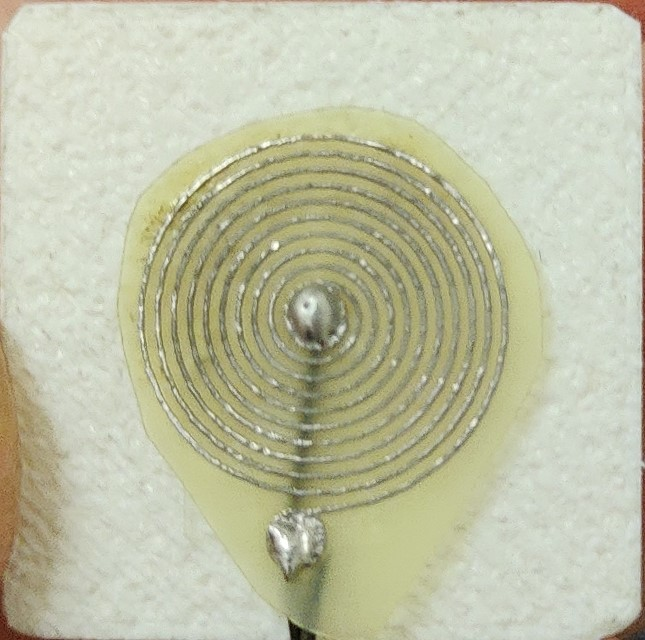
\includegraphics{Chapters/Chapter5/Figures/Dresden_coil.jpg}}
    \caption{Dresden coil \cite{HZDR}}
    \label{fig:Dresden_coil}
\end{figure}

\subsubsection{Low resistance and high power needs}
The Dresden coils have a \textbf{resistance} of about \textbf{2$\Omega$}, \textbf{external radius} of \textbf{5e-3m}, \textbf{internal} one of \textbf{0.84*e-3m}, and \textbf{number of spires} equal to \textbf{11}.
We also know from the HZDR test that the coil can handle up to about \textbf{500mA} before starting to release too much heat.
This means a power limit of about \textbf{0.5W} for the coil.

The current limit is due to the very low resistance of the coil as due to this limitation, for low applied voltages the coil will produce a lot of heat due to the Joule effect \ref{subsubsec: Joule_effect}.

\begin{figure}
    \centering
    \resizebox{0.5\textwidth}{!}{\begin{tikzpicture}
    \begin{axis}[
            xmin=0, ymin=0, xmax=3, ymax=2.5, samples=500,
            xlabel={Voltage [$V_{rms}$]},ylabel={Power [$W$]}, title={Power output vs $V_{rms}$}
        ]

        \addplot[blue, thick, domain=0:8, name path=func] (x, x^2/2);
        \addplot[red, thick, name path=limit] coordinates {
            (sqrt(0.5*2), \pgfkeysvalueof{/pgfplots/ymin}) 
            (sqrt(0.5*2), \pgfkeysvalueof{/pgfplots/ymax})
        }; % vertical limit line 

        \path[name path=axis] (axis cs:\pgfkeysvalueof{/pgfplots/xmin},0) -- (axis cs:\pgfkeysvalueof{/pgfplots/xmax},0);
        \path[name path=vend] (axis cs:\pgfkeysvalueof{/pgfplots/xmax},\pgfkeysvalueof{/pgfplots/ymin}) -- (axis cs:\pgfkeysvalueof{/pgfplots/xmax},\pgfkeysvalueof{/pgfplots/ymax});

        \addplot[red!25] fill between [of = limit and vend];
        % TODO: Add label to the limit line and legend
    \end{axis}
\end{tikzpicture}}
    \caption{Power profile of the Dresden coil}
    \label{fig: Dresden_heat_graph}
\end{figure}
As we can see in figure \ref{fig: Dresden_heat_graph}, after 1V the power limit is already reached.

\subsubsection{Low magnetic field strength}
For the same reason as the power limit, the magnetic field produced by the Dresden coil is very low.
Using the equation \ref{eq:Spiral_magn_field_eq} we can calculate the magnetic field produced by the Dresden coil on its surface and plot it as a function of the voltage applied to the coil.
\begin{figure}
    \centering
    \resizebox{0.5\textwidth}{!}{\begin{tikzpicture}
    \begin{axis}[
            xmin=0, ymin=0, xmax=1, ymax=8e-3, samples=500,
            xlabel={Power [$P_{rms}$]},ylabel={Magnetic Field [$T$]}, title={Magnetic Field vs $P_{rms}$}
        ]

        \addplot[blue, thick, domain=0:3.5, name path=func] (x, 0.0021*x^0.5);
        \addplot[red, thick, name path=limit] coordinates {
            (0.5, \pgfkeysvalueof{/pgfplots/ymin}) 
            (0.5, \pgfkeysvalueof{/pgfplots/ymax})
        }; % vertical limit line 

        \path[name path=axis] (axis cs:\pgfkeysvalueof{/pgfplots/xmin},0) -- (axis cs:\pgfkeysvalueof{/pgfplots/xmax},0);
        \path[name path=vend] (axis cs:\pgfkeysvalueof{/pgfplots/xmax},\pgfkeysvalueof{/pgfplots/ymin}) -- (axis cs:\pgfkeysvalueof{/pgfplots/xmax},\pgfkeysvalueof{/pgfplots/ymax});

        \addplot[red!25] fill between [of = limit and vend];
        % TODO: Add label to the limit line and legend
    \end{axis}
\end{tikzpicture}}
    \caption{Magnetic field produced by the Dresden coil}
    \label{fig: Dresden_magnetic_field}
\end{figure}

As we can see in figure \ref{fig: Dresden_magnetic_field}, even at the power limit, the magnetic field produced by the Dresden coil is very low (in the order of 1mT).

\subsubsection{Fragility and low flexibility}
The Dresden coil is produced by using three layers of different materials.
The first layer is the substrate, which is made of a material similar to paper, the second layer is the conductive ink, and the third layer is the tinning.
The substrate is not very flexible, and neither is the tinning;
this makes the spires of the coil easily damageable if bent repeatedly.
Also, the tinning gets cracked by repeatedly heating and cooling the coil, which constantly happens during the coil's use.
The tinning cracking would happen multiple times during our tests, and we would have to re-tin the damaged parts of the coil to keep using it.




% -- Subsection 5.2
\subsection{Flexar coils}
Flexar coils are flexible PCB coils designed by the independent researcher Carl Bugeja \cite{Carl_Bugeja}.
He designed these very thin flexible coils intending to use them to actuate very small robots and lightweight objects.
This characteristic comes at the cost of not being able to produce very high magnetic fields.
We will be using for this research an old model of the Flexar coil that precedes the opening of the company \textbf{microbots} \cite{microbots}.
\begin{figure}
    \centering
    \resizebox{0.5\textwidth}{!}{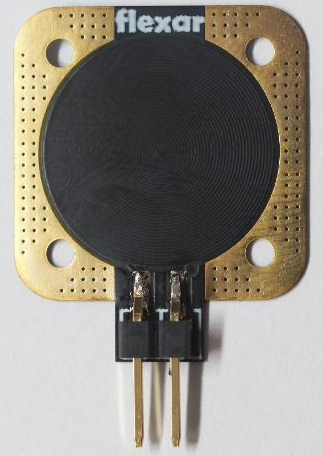
\includegraphics{Chapters/Chapter5/Figures/Flexar_coil.png}}
    \caption{Flexar coil }
    \label{fig:Flexar_coil}
\end{figure}


\subsubsection{Lower resistance and power needs}
We previously discussed the Flexar coil's characteristics in section \ref{subsec: Application challenges}.
But to sum up they have a \textbf{resistance} of about \textbf{30$\Omega$}, \textbf{external radius} of \textbf{6.86e-3m}, \textbf{internal} one of about \textbf{1e-4m}, and \textbf{number of spires} equal to \textbf{70} (composed of two coils of 35 in series).
It can handle up to about \textbf{0.8W} before starting to release too much heat.

We report here the same graph as the previously cited section:
\begin{figure}
    \centering
    \resizebox{0.5\textwidth}{!}{\begin{tikzpicture}
    \begin{axis}[
            xmin=0, ymin=0, xmax=8, ymax=2.5, samples=500,
            xlabel={Voltage [$V_{rms}$]},ylabel={Power [$W$]}, title={Power output vs $V_{rms}$}
        ]

        \addplot[blue, thick, domain=0:8, name path=func] (x, x^2/30);
        \addplot[red, thick, name path=limit] coordinates {
            (sqrt(0.8*30), \pgfkeysvalueof{/pgfplots/ymin}) 
            (sqrt(0.8*30), \pgfkeysvalueof{/pgfplots/ymax})
        }; % vertical limit line 

        \path[name path=axis] (axis cs:\pgfkeysvalueof{/pgfplots/xmin},0) -- (axis cs:\pgfkeysvalueof{/pgfplots/xmax},0);
        \path[name path=vend] (axis cs:\pgfkeysvalueof{/pgfplots/xmax},\pgfkeysvalueof{/pgfplots/ymin}) -- (axis cs:\pgfkeysvalueof{/pgfplots/xmax},\pgfkeysvalueof{/pgfplots/ymax});

        \addplot[red!25] fill between [of = limit and vend];
        % TODO: Add label to the limit line and legend
    \end{axis}
\end{tikzpicture}}
    \caption{Power profile of the Flexar coil}
    \label{fig: Flexar_heat_graph}
\end{figure}

As we can see in figure \ref{fig: Flexar_heat_graph}, the Flexar coil can handle more power than the Dresden coil.

\subsubsection{Higher magnetic field strength}
Due to their characteristics, Flexar coils can produce higher magnetic fields than the Dresden coil but not unlike them, they are still limited by the power they can handle.
\begin{figure}
    \centering
    \resizebox{0.5\textwidth}{!}{\begin{tikzpicture}
    \begin{axis}[
            xmin=0, ymin=0, xmax=1, ymax=8e-3, samples=500,
            xlabel={Voltage [$V_{rms}$]},ylabel={Magnetic Field [$T$]}, title={Magnetic Field vs $V_{rms}$}
        ]

        \addplot[blue, thick, domain=0:8, name path=func] (x, 0.005*x^0.5);
        \addplot[red, thick, name path=limit] coordinates {
            (0.8, \pgfkeysvalueof{/pgfplots/ymin}) 
            (0.8, \pgfkeysvalueof{/pgfplots/ymax})
        }; % vertical limit line 

        \path[name path=axis] (axis cs:\pgfkeysvalueof{/pgfplots/xmin},0) -- (axis cs:\pgfkeysvalueof{/pgfplots/xmax},0);
        \path[name path=vend] (axis cs:\pgfkeysvalueof{/pgfplots/xmax},\pgfkeysvalueof{/pgfplots/ymin}) -- (axis cs:\pgfkeysvalueof{/pgfplots/xmax},\pgfkeysvalueof{/pgfplots/ymax});

        \addplot[red!25] fill between [of = limit and vend];
        % TODO: Add label to the limit line and legend
    \end{axis}
\end{tikzpicture}}
    \caption{Magnetic field produced by the Flexar coil}
    \label{fig: Flexar_magnetic_field_vs_P}
\end{figure}
As we can observe in figure \ref{fig: Flexar_magnetic_field_vs_P}, the Flexar coil, at the power limit of the Dresden coil, can produce a higher magnetic field (in the order of 2.5mT).
This proves that the Flexar coil is more capable than the Dresden coil in producing magnetic fields but even at its power limit the field produced is still feeble (it is in the order of \textbf(4mT)).

\subsubsection{Higher flexibility}
Flexible PCBs are made of a substrate of polyimide, which is a very flexible material.
It can withstand being bent at a very tight radius multiple times without breaking.

Between the layers of polyimide, we have the copper traces that don't require any tinning to work.
This makes the Flexar coil more durable than the Dresden coil, as it doesn't have any parts that can crack due to bending or heating and cooling.

Also, we observed that the Flexar coil can withstand temperatures in exceed of 100$^{\circ}$C.

